\tikzset{>=latex} % for LaTeX arrow head

\colorlet{myblue}{blue!20}
\colorlet{mydarkblue}{blue!50!black}
\colorlet{myred}{black!50!red}

\tikzset{
  cube/.pic={
    \tikzset{every edge quotes/.append style={midway,auto},/cube/.cd,#1}
    \def\csize{2*\cubesize}
    \draw [every edge/.append style={pic actions,densely dashed,opacity=.5},pic actions]
    (0,0,0) coordinate (o)
            edge coordinate [pos=1] (g) ++(0,0,-\csize)
        --++(0,\csize,0) coordinate (a)
        --++(\csize,0,0) coordinate (b)
        --++(0,-\csize,0) coordinate (c) -- cycle
    (a) --++(0,0,-\csize) coordinate (d) edge (g)
        --++(\csize,0,0) coordinate (e) -- (b) -- cycle
    (c) -- (b) -- (e)
        --++(0,-\csize,0) coordinate (f) edge (g) -- cycle;
    \path [every edge/.append style={pic actions, |-|}];
  },
  z={(-0.334,-0.334)},
  /cube/.search also={/tikz},
  /cube/.cd,
  size/.store in=\cubesize, size=1,
}

\tikzset{
  gasparticle/.pic={
    \tikzset{/gasparticle/.cd,#1}
    \draw[->,green!60!black] (0,0) -- (\vec);
    \node[circle,fill,inner sep=.8,fill=black!80!blue] at (0,0,0) {};
  }
  /gasparticle/.search also={/tikz},
  /gasparticle/.cd,
  vec/.store in=\vec, vec={90:0.5},
}

% GAS in a box



% GAS in a box - partioned


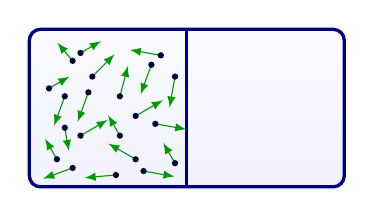
\begin{tikzpicture}
  \draw[mydarkblue,very thick,rounded corners=4,
        top color=blue!2,bottom color=blue!5,shading angle=0]
    (0,0) rectangle (4,2);
  \draw[mydarkblue,very thick] (2,0) --++ (0,2);
  %\draw[blue!50,dashed] (1,0) --++ (0,2);
  %\draw[blue!50,dashed] (3,0) --++ (0,2);
  %\draw[blue!50,dashed] (0,1) --++ (4,0);
  %\draw[blue!50,dashed] (0,0.5) --++ (4,0);
  %\draw[blue!50,dashed] (0,1.5) --++ (4,0);
  \pic at (0.25,1.25) {gasparticle={vec={  30:0.3}}};
  \pic at (0.35,0.35) {gasparticle={vec={ 120:0.3}}};
  \pic at (0.45,1.15) {gasparticle={vec={-110:0.4}}};
  \pic at (0.45,0.75) {gasparticle={vec={ -80:0.3}}};
  \pic at (0.55,0.24) {gasparticle={vec={-160:0.4}}};
  \pic at (0.55,1.60) {gasparticle={vec={ 130:0.3}}};
  \pic at (0.65,0.65) {gasparticle={vec={  30:0.4}}};
  \pic at (0.65,1.70) {gasparticle={vec={  30:0.3}}};
  \pic at (0.80,1.40) {gasparticle={vec={  45:0.4}}};
  \pic at (0.75,1.20) {gasparticle={vec={-110:0.4}}};
  \pic at (1.10,0.15) {gasparticle={vec={-175:0.4}}};
  \pic at (1.15,0.65) {gasparticle={vec={ 120:0.3}}};
  \pic at (1.15,1.15) {gasparticle={vec={  75:0.4}}};
  \pic at (1.35,0.90) {gasparticle={vec={  30:0.4}}};
  \pic at (1.35,0.35) {gasparticle={vec={ 150:0.4}}};
  \pic at (1.45,0.20) {gasparticle={vec={ -10:0.4}}};
  \pic at (1.55,1.55) {gasparticle={vec={-110:0.4}}};
  \pic at (1.60,0.80) {gasparticle={vec={ -10:0.4}}};
  \pic at (1.67,1.67) {gasparticle={vec={ 170:0.4}}};
  \pic at (1.85,0.30) {gasparticle={vec={ 120:0.3}}};
  \pic at (1.85,1.40) {gasparticle={vec={-100:0.4}}};
\end{tikzpicture}
